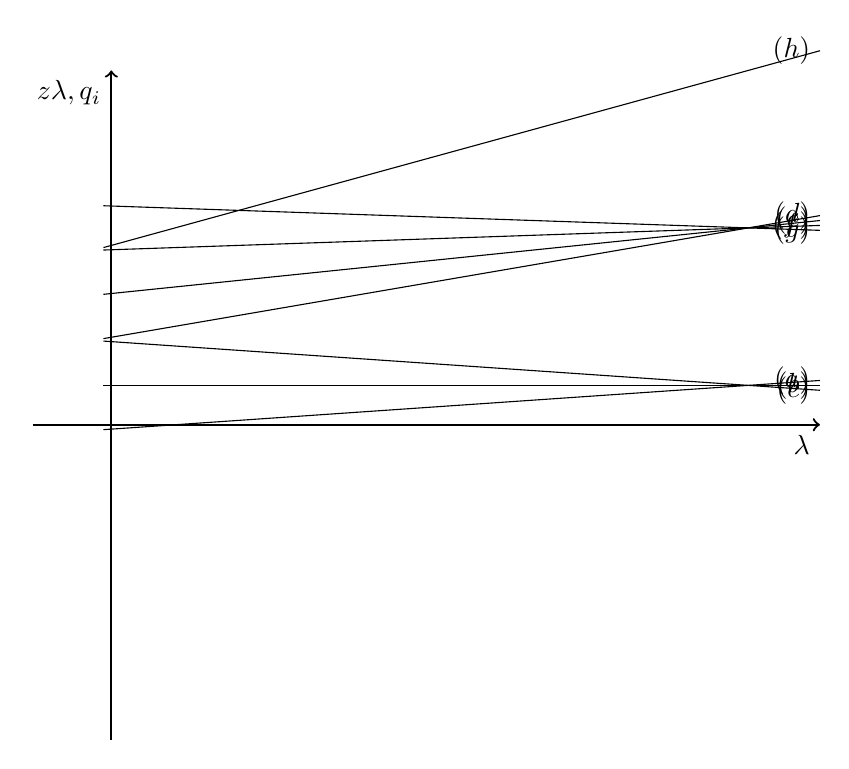
\begin{tikzpicture}[xscale=8,yscale=0.25]
\draw[thick,->] (-0.125,18) -- (1.125,18) node[anchor=north east]{$\lambda$};
\draw[thick,->] (0,2) -- (0,36) node[anchor=north east]{$\fun{z}{\lambda,q_i}$};
\foreach \i/\b/\a in {a/18/2,b/20/0,c/22/-2,d/23/5,e/25/3,f/27/1,g/29/-1,h/28/8} {
  \draw (-0.0125,-0.125*\a+\b) -- (1.125,1.125*\a+\b) node[anchor=east] {$(\i)$};
}
\end{tikzpicture}